%
% teil1.tex -- Beispiel-File für das Paper
%
% (c) 2020 Prof Dr Andreas Müller, Hochschule Rapperswil


\section{Lösungsmethode 1: Separationsmethode 
	\label{kreismembran:section:teil1}}
\rhead{Lösungsmethode 1: Separationsmethode}
An diesem Punkt bleibt also nur noch die Lösung der partiellen Differentialgleichung. In diesem Abschnitt wird sie mit Hilfe der Separationsmethode gelöst.

\subsection{Aufgabestellung\label{sub:aufgabestellung}}
Wie im vorherigen Abschnitt gezeigt, lautet die partielle Differentialgleichung, die die Schwingungen einer Membran beschreibt:
\begin{equation*}
	\frac{1}{c^2}\frac{\partial^2u}{\partial t^2} = \Delta u.
\end{equation*}
Da es sich um eine Kreisscheibe handelt, werden Polarkoordinaten verwendet, so dass sich der Laplaceoperator
\begin{equation*}
	\Delta
	=
	\frac{\partial^2}{\partial r^2}
	+
	\frac1r
	\frac{\partial}{\partial r}
	+
	\frac{1}{r^2}
	\frac{\partial^2}{\partial\varphi^2}
	\label{buch:pde:kreis:laplace}
\end{equation*}
ergibt.

Es wird eine runde elastische Membran berücksichtigt, die das Gebiet $\Omega$ abdeckt und am Rand $\Gamma$ befestigt ist.
Es wirken keine äusseren Kräfte. Es handelt sich somit von einer kreisförmligen eingespannten homogenen schwingenden Membran nach den Annahmen von \ref{kreimembran:annahmen}.

Daher ist die Membranabweichung im Punkt $(r,\varphi)$ $\in$ $\overline{\rm \Omega}$ zum Zeitpunkt $t$:
\begin{align*}
	u: \overline{\rm \Omega} \times \mathbb{R}_{\geq 0} &\longrightarrow \mathbb{R}\\
	(r,\varphi,t) &\longmapsto u(r,\varphi,t)
\end{align*}
Um die Vergleichbarkeit der beiden nachfolgend vorgestellten Lösungsverfahren in Abschnitt \ref{kreismembran:vergleich} zu vereinfachen, werden keine Randbedingungen vorgegeben.

Um eine eindeutige Lösung bestimmen zu können, werden die folgenden Anfangsbedingungen festgelegt zur Zeit $t = \text{0}$:
\begin{align*}
	u(r,\varphi, 0) &= f(r,\varphi)\\
	u_t(r,\varphi, 0) &= g(r,\varphi).
\end{align*}

\subsection{Lösung\label{sub:lösung1}}
Nun wird das in Abschnitt \ref{sub:aufgabestellung} vorgestellte Problem mit Hilfe der Separationsmethode gelöst.
\subsubsection{Ansatz der Separation der Variablen\label{subsub:ansatz_separation}}
Hierfür wird folgenden Ansatz gemacht:
\begin{equation*}
	u(r,\varphi, t) = F(r)G(\varphi)T(t)
\end{equation*}
Dank der Randbedingungen kann gefordert werden, dass $F(R)=0$ ist, und natürlich, dass $G(\varphi)$ $2\pi$ periodisch ist. Eingesetzt in der Differenzialgleichung ergibt sich:
\begin{equation*}
	\frac{1}{c^2}\frac{T''(t)}{T(t)}=-\kappa^2=\frac{F''(r)}{F(r)}+\frac{1}{r}\frac{F'(r)}{F(r)}+\frac{1}{r^2}\frac{G''(\varphi)}{G(\varphi)}.
\end{equation*}
Da die linke Seite nur von $t$ und die rechte Seite nur von $r$ und $\varphi$ abhängt, müssen sie gleich einer reellen Zahl sein. 
Laut Annahme iv) in \ref{kreimembran:annahmen} erfährt die Membran keine Dämpfung.
Daher werden Lösungen gesucht, die weder exponentiell in der Zeit wachsen noch exponentiell abklingen. 
Dies bedeutet, dass die Konstante negativ sein muss, also schreibt man $-\kappa^2$. Daraus ergeben sich die folgenden zwei Gleichungen:
\begin{align*}
	T''(t) + c^2\kappa^2T(t) &= 0\\
	r^2\frac{F''(r)}{F(r)} + r \frac{F'(r)}{F(r)} +\kappa^2 r^2 &= - \frac{G''(\varphi)}{G(\varphi)}.
\end{align*}
In der zweiten Gleichung hängt die linke Seite nur von $r$ ab, während die rechte Seite nur von $\varphi$ abhängt. Sie müssen also wiederum gleich einer reellen Zahl $\nu$ sein. Also:
\begin{align*}
	r^2F''(r) + rF'(r) + (\kappa^2 r^2 - \nu)F(r) = 0 \quad \text{und} \quad
	G''(\varphi) = \nu G(\varphi).
\end{align*}

\subsubsection{Lösung für $G(\varphi)$\label{subsub:lösung_G}}
Da für die zweite Gleichung Lösungen von Schwingungen erwartet werden, für die $G''(\varphi)=-\omega^2 G(\varphi)$ gilt, schreibt man die gemeinsame Konstante als $\nu=-\omega^2$, was die Formeln später vereinfacht. Also:
\begin{equation*}
 G(\varphi) = C_n \cos(\nu\varphi) + D_n \sin(\nu\varphi)
 \label{eq:cos_sin_überlagerung}
\end{equation*}

\subsubsection{Lösung für $F(r)$\label{subsub:lösung_F}}
Die Gleichung für $F$ hat die Gestalt (Verweis auf \label{buch:differentialgleichungen:bessel-operator}
\begin{align}
	r^2F''(r) + rF'(r) + (\kappa^2 r^2 - n^2)F(r) = 0 
	\label{eq:2nd_degree_PDE}
\end{align}
Wir bereits in Kapitel \ref{buch:differntialgleichungen:section:bessel} gezeigt, sind die Bessel-Funktionen
\begin{equation*}
	J_{\nu}(x) = r^\nu \displaystyle\sum_{m=0}^{\infty} \frac{(-1)^m x^{2m}}{2^{2m+\nu}m! \Gamma (\nu + m+1)}
\end{equation*}
Lösungen der Besselschen Differenzialgleichung
\begin{equation*}
	x^2 y'' + xy' + (\kappa^2 - \nu^2)y = 0
\end{equation*}
Die Funktionen $F(r) = J_n(\kappa r)$ lösen die Differentialgleichung \eqref{eq:2nd_degree_PDE}.

\subsubsection{Lösung für $T(t)$\label{subsub:lösung_T}}
Die Differenzialgleichung $T''(t) + c^2\kappa^2T(t) = 0$, wird auf ähnliche Weise gelöst wie $G(\varphi)$. 

\subsubsection{Zusammenfassung der Lösungen\label{subsub:zusammenfassung_lösungen}}
Durch Überlagerung aller Ergebnisse erhält man die Lösung
\begin{align}
	u(r, \varphi, t) = \displaystyle\sum_{m=1}^{\infty}\displaystyle\sum_{n=0}^{\infty} J_n (k_{mn}r)[a_{mn}\cos(n\varphi) + b_{mn}\sin(n\varphi)](n\varphi)[c_{mn}\cos(c \kappa_{mn} t)+d_{mn}\sin(c \kappa_{mn} t)]
	\label{eq:lösung_endliche_generelle}
\end{align}

Dabei sind $m$ und $n$ ganze Zahlen, wobei $m$ für die Anzahl der Knotenkreise und $n$
für die Anzahl der Knotenlinien steht. Es gibt bestimmte Bereiche auf der Membran, in denen es keine Bewegung oder Vibration gibt. Wenn der nicht schwingende Bereich ein Kreis ist, nennt man ihn einen Knotenkreis, und wenn er eine Linie ist, nennt man ihn ebenfalls eine Knotenlinie (siehe Abbildung \ref{buch:pde:kreis:fig:pauke}). $J_n(\kappa_{mn}r)$ ist die Besselfunktion $n$-ter Ordnung, wobei $\kappa mn$ die Wellenzahl und $r$ der Radius ist. $a_{mn}$ und $b_{mn}$ sind die zu bestimmenden Konstanten.

\begin{figure}
	\centering
	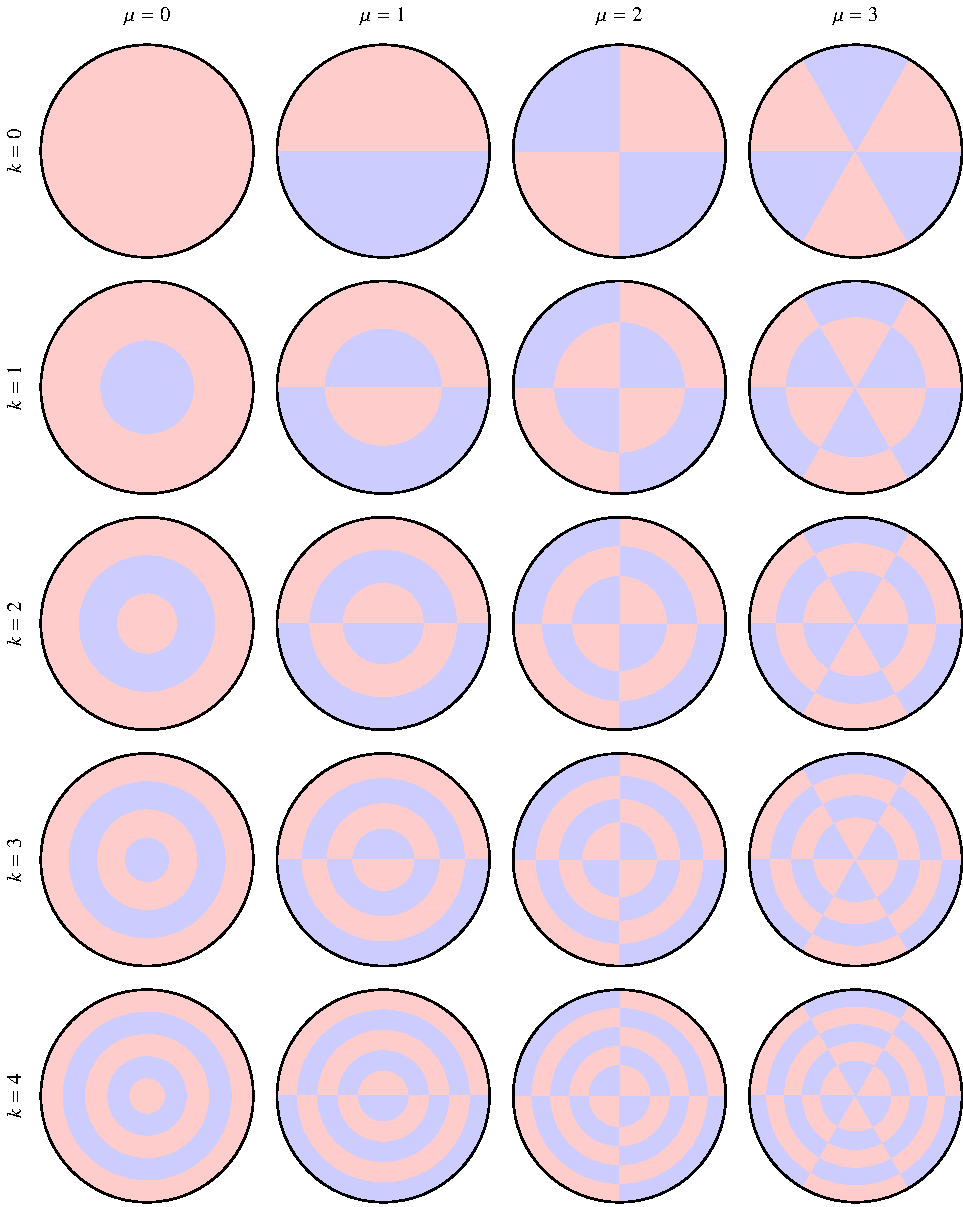
\includegraphics[width=\textwidth]{chapters/090-pde/bessel/pauke.pdf}
	%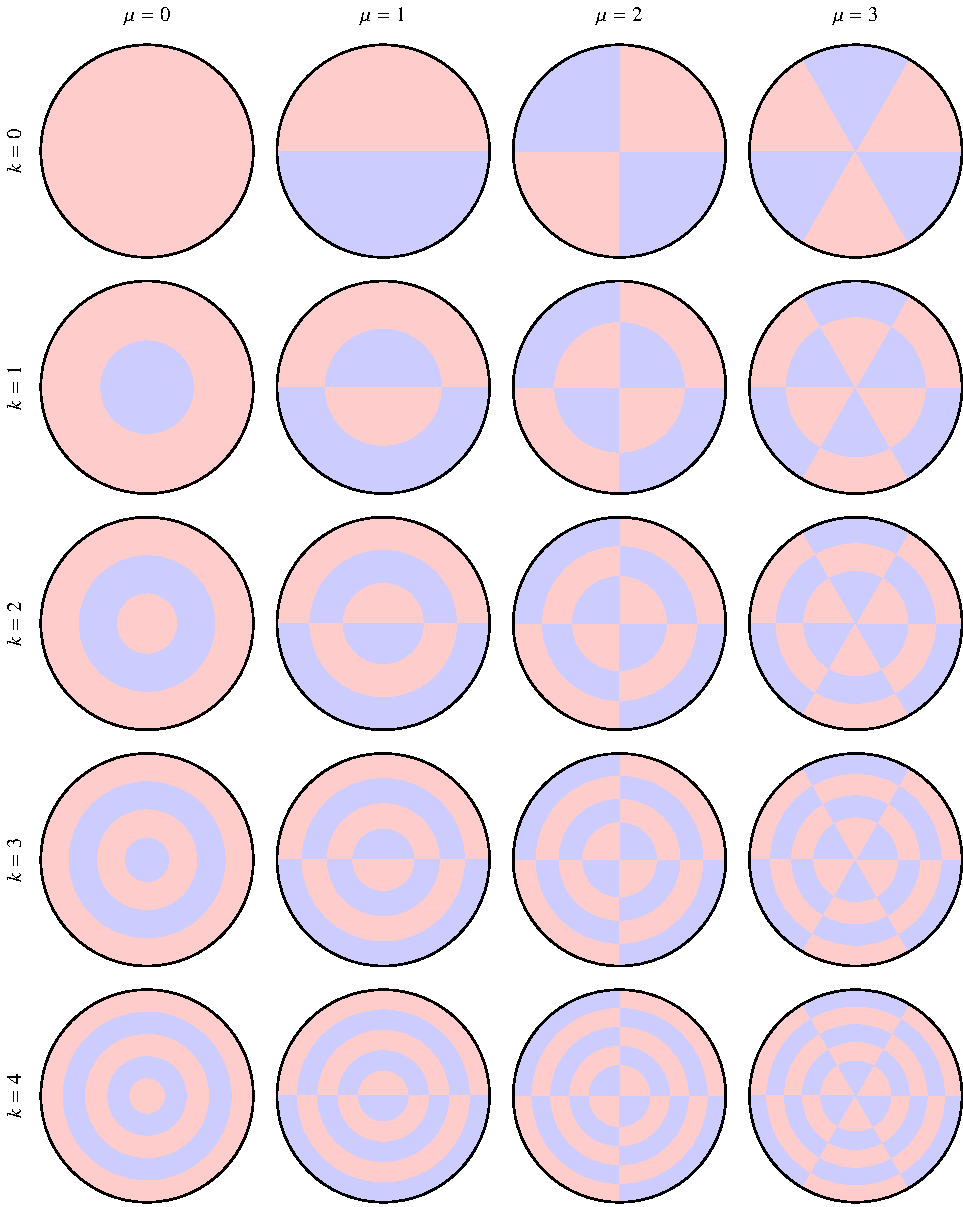
\includegraphics{chapters/090-pde/bessel/pauke.pdf}
	\caption{Vorzeichen der Lösungsfunktionen und Knotenlinien
		für verschiedene Werte von $\mu$ und $k$.
		Die Bereiche, in denen die Lösungsfunktion positiv sind, ist 
		rot dargestellt, die negativen Bereiche blau.
		In jeder Darstellung gibt es genau $k+\mu$ Knotenlinien.
		Die Radien der kreisförmigen Knotenlinien müssen aus den Nullstellen
		der Besselfunktionen berechnet werden.
		\label{buch:pde:kreis:fig:pauke}}
\end{figure}


An diesem Punkt stellte sich die Frage, ob es möglich wäre, die partielle Differentialgleichung mit einer anderen Methode als der der Trennung der Variablen zu lösen. Nach einer kurzen Recherche wurde festgestellt, dass eine weitere Methode die Transformationsmethode ist, genauer gesagt die Anwendung der Hankel-Transformation. Im nächsten Kapitel wird daher diese Integraltransformation vorgestellt und entwickelt, und es wird erläutert, warum sie für diese Art von Problem geeignet ist.
